\documentclass[preprint,aps,floatfix,showpacs]{revtex4-2}
%\documentclass[aps,twocolumn,showpacs,floatfix]{revtex4-2}
%\documentclass[aps,twocolumn,showkeywords,floatfix,superscriptaddress]{revtex4-1}
\usepackage{dcolumn,multirow}
\usepackage{graphicx}
%\usepackage{graphics}
\usepackage{amsfonts,mathtools,amsmath,bm,amssymb}
\usepackage{comment}
%\usepackage[utf8]{inputenc} 
%\usepackage[utf8x]{inputenc}
\usepackage[usenames]{color}
\usepackage[flushleft]{threeparttable}
\usepackage{titlesec}
\usepackage{etoolbox} % for \appto
\usepackage{lipsum} % for mock text
\usepackage[capitalize]{cleveref}
\usepackage{makecell}
\usepackage[section]{placeins}
\usepackage{float}
\usepackage{color}
\newcommand{\red}[1]{\textcolor{red}{#1}}
\newcommand{\blue}[1]{\textcolor{blue}{#1}}
\newcommand{\green}[1]{\textcolor{green}{#1}}
\usepackage[T1]{fontenc}
\usepackage{textcomp}
\usepackage[utf8]{inputenc}
\DeclareUnicodeCharacter{00B2}{\ensuremath{{}^2}}

\begin{document}
\title{Deep learning model for predicting material composition from X-ray photoelectron spectroscopy data }
\author{In-Ho Lee} %\email{ihlee@kriss.re.kr}
\affiliation{Korea Research Institute of Standards and Science, Daejeon 34113, Korea}
\author{J. H. Choi} 
\author{Yongsup Park} \email[corresponding author ]{parky@khu.ac.kr}
\affiliation{Department of Physics, Kyung Hee University, Seoul 02447, Korea}
\date{\today }
	

\begin{abstract}
We develop a deep learning model to infer material composition from X-ray photoelectron spectroscopy data and test its performance.
We generate a synthetic dataset made of 75000 spectra based on XPS parameter databases and electron scattering theory in the transport approximation. We considered 2, 3, 4, and 5 as the different types of atoms a substance can have.
We use synthetic data for the X-ray photoelectron spectroscopy model development and utilize the latest artificial intelligence techniques to build a model that can predict the degree of carbon contamination and composition. 
The mean absolute error in the carbon contamination prediction for the test dataset is 14.5\%. 
In addition, the mean of the maximum absolute error for the composition ratio prediction is 6.4\%.

\end{abstract}
%\pacs{02.60.Cb, 89.20.Bb, 84.40.Ua}% PACS, the Physics and Astronomy Classification Scheme.
\keywords{X-ray photoelectron, deep learning, chemical composition}%Use showkeys class option if keyword display desired
\maketitle
\newpage

\section{Introduction} \label{introduction}
X-ray photoelectron spectroscopy(XPS) method is widely used in characterizing materials.
XPS analysis is the measurement of the composition and atomistic bonding properties of materials.
By irradiating a sample with X-rays we obtain the kinetic energy and intensity of photoelectrons emitted 
by the photoelectric effect\cite{fadley2010x}.
X-ray energy can be absorbed by one of the core electrons. 
The energy needed to cause the core electron to be emitted 
and subsequently detected is characteristic to each element. 
This characteristic feature allows the use of binding energy to identify the elements present on the surface of the material.
Peak intensity at a specific binding energy 
usually displays the total number of photoelectron counts per second. 
Sometimes there would be an overlapping peaks, unresolved peaks on the binding energy axis.
Specifically, it is important to check the core-levels and Auger-lines for each atom. 

XPS can detect all elements except hydrogen and helium with detection
limits of approximately 0.1\%–1\%.
Since XPS is extremely surface sensitive, care must be taken to avoid surface contamination.
Since each element has its own unique binding energy, comparing the peaks and binding energies in the spectrum can be used to determine the composition of the elements present on the sample surface.
Binding energy is characteristic of the chemical environment of the core-excited atom, corresponding structural characterization.
Also, when the chemical bonding state of an atom changes, the binding energy usually changes by a few eV, so the chemical bonding state can be inferred from this change. 
In addition, XPS simultaneously provides chemical information on the chemical structure, degree of carbon contamination, and oxidation state of the sample component atoms. 
Computational prediction of core-electron binding energies is also developed\cite{golze2022accurate,sun2022machine}.



%The information about existing bonds is typically extracted by comparing measured binding energy values to literature data bases\cite{crist2019xps}.

XPS results can be challenging to interpret, in general, although there is a data base for binding energy values\cite{chastain1992handbook,crist2019xps}. 
Sometimes XPS data are often misinterpreted in the literature. 
Many factors in the experiment affect binding energies in XPS method. 
The binding energies of different atomic features can even overlap, further complicating the analysis.
In fact, generation of photoelectrons is closely related to processes that result from x-ray bombardment of a surface include emission of a photoelectron,  x-ray fluorescence, and emission of an Auger electron.

By obtaining a variety of experimental measurement data, it is possible to understand the general XPS measurement data.  
It is also possible to infer XPS spectra of materials with arbitrary compositions from sufficient data.
This is known as the traditional XPS analysis and is widely utilized in both materials physics and industrial researches. 
Similarly, research has recently been conducted on inferring composition ratios using deep learning method\cite{drera2020deep}. It can be seen that the ability to make inferences from data can be achieved through machine learning. 

Recent advances in artificial intelligence have made it possible to make systematic inferences that have never been easily attempted before\cite{goodfellow2016deep}. In this work, we developed and tested a model for correlating XPS data with chemical composition using probabilistic inference supported by recent machine learning methods. 
At this point, it would be natural to try to leverage artificial intelligence to build models for predicting carbon contamination and composition ratio that are as accurate as those of long-time experts.

Section \ref{methods} provides machine learning details. Section \ref{results} presents and discusses model performance. 
Finally, Section \ref{conclusions} concludes the paper.

\section{Methods} \label{methods}
For training and validation, we use the in silico-generated dataset. 
It is possible to generate synthetic dataset for XPS by taking into account composition and carbon contamination. 
The network was trained on the simulated dataset.


\subsection{synthetic data}
We generated a synthetic dataset made of 75000 spectra based on XPS parameter databases and electron scattering theory in the transport approximation\cite{werner2001electron}. 
Only Al k$_{\alpha}$ source is used.
Each detail of real XPS spectra, including peak position, intensity, inelastic loss backgrounds, chemical shifts, the analyzer transmission function, and the signal-to-noise ratio has been carefully simulated according to available XPS databases and theories.
The spectra kinetic energy range was 400–1486 eV on a 2048 energy point grid. 

We consider random possible combinations of elements 
from the list of Li, Be, B, C, ..., and Bi atoms. 
Each virtual material is composed by a random number(from 2 to 5) of elements, with variable stoichiometry ratios.
The carbon contamination leads to an overall lower XPS intensity\cite{evans1997correction}.

The training dataset size is 75000.
The validation dataset size and test dataset size are 600 and  3000, respectively.
The present network takes as input the 2048 spectral points $(\{x_j\}, j = 1, \ldots, 2048.)$ and produces two outputs, the normalized carbon contamination level $c (0 \le c \le 1)$ and the normalized intensity $(\{y_e\}, 0 \le y_e \le 1, e = 1, \ldots, 81.)$ of the 81 element.


\subsection{deep learning model}
The single neural network we used predicts each of the two by itself. The first is the degree of carbon contamination($0 \le c \le 1$) and the second is the composition ratio( $0 \le y_e \le 1$, $e=1, 2, 3, \ldots, 81$). As explained earlier, H and He are excluded from the study.
We built a model that simultaneously optimizes the regression(contamination degree) and regression(composition ratio) loss functions using multiple one-dimensional convolutional nueral network layers, multihead attention layer, dense layers, and dropout layers. 
Our model is based on TensorFlow.
A `softmax' activation function for the final layer is used to normalize the outputs so that ${\sum }_{e=1}^{81}{y}_{e}=1$.
An `adam' optimizer\cite{kingma2014adam} and the tuned loss function allowed for a robust training.
A `sigmoid' activation, is used to identify the level of carbon contamination $c$.
Total number of trainable parameters is  8765675.

\subsection{loss functions}
Mean squared logarithmic error($MSLE$) is considered to be an improvement over using percentage based errors for training because its numerical properties are better.
\begin{equation}
	MSLE(\{y_e\}, \{y_e^t\}) = \frac{1}{81} \sum_{e=1}^{81}\left\{log(1+y_e)-log(1+y^t_e)  \right\}^2,
	\label{eq:msle}
\end{equation}
where $\{y_e\}$ are the network outputs and $\{y_e^t\}$ the target values. 
It is less sensitive to outliers than mean squared error since the logarithmic transformation compresses the error values.
The loss function is scale independent as it is a difference of two log values which is the same as log of the ratio of the values. 
Due to the loss being log it penalizes underestimates more than overestimates.


\subsection{training and validation}
We plotted the loss functions over the training epoch in the Fig. \ref{conv}. We also plotted the loss functions for the validation dataset on the model at the same time. The loss functions are related to the prediction of the degree of carbon contamination and the prediction of the composition ratio, respectively.


 
The mean absolute error($\mid c-c^t \mid$, $0\le c \le1$. $c$, $c^t$ are predicted carbon contamination value and true carbon contamination value, respectively.) in the carbon contamination prediction for the test dataset(sample size: 1000) is 0.145. 
For the same test dataset, the mean of the maximum absolute error($max\mid y_e-y^t_e\mid$, $0 \le y_e \le 1$) for the composition ratio prediction is 0.064.

\section{Results and discussion} \label{results}


\section{Conclusions}	\label{conclusions}
To summarize, we developed an accurate and efficient deep learning model to infer material composition from XPS data.  We have shown that the model we built has expert-level predictive capabilities and can be used to infer  composition and carbon contamination as the simplest application. 
We generated a synthetic dataset made of 75000 spectra based on XPS parameter databases and electron scattering theory in the transport approximation.  We considered 2, 3, 4, and 5 as the different types of atoms a substance can have.
The mean absolute error in the carbon contamination prediction for the test dataset is 14.5\%. 
In addition, the mean of the maximum absolute error for the composition ratio prediction is 6.4\%.	
	
~\\
%\section{Acknowledgments} 
This research was supported by Enhancement of Measurement
Standards and Technologies in Physics funded by Korea Research
Institute of Standards and Science (No. KRISS-2021-GP2021-0002).

\bibliography{myref}

\newpage


\begin{figure}
	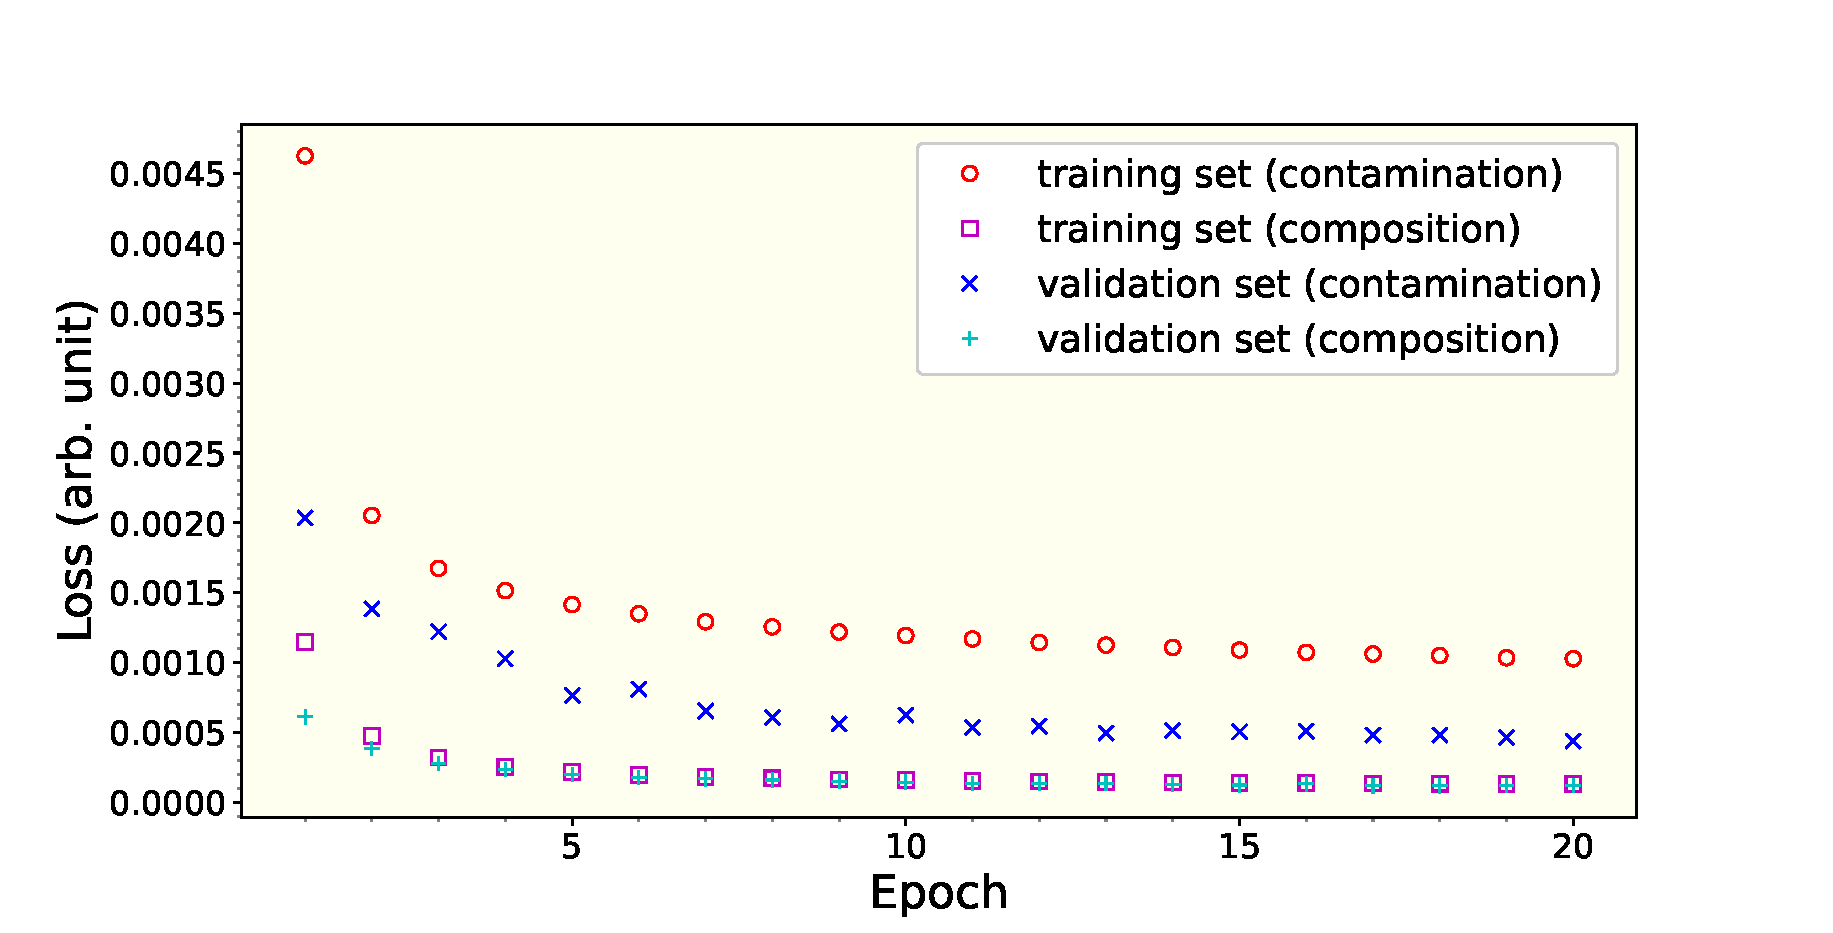
\includegraphics[width=1.1\columnwidth]{conv1.eps}
	\caption{The loss functions are related to the prediction of the degree of carbon contamination and the prediction of the composition ratio, respectively. Mean squared logarithmic error($MSLE$) is used for both contamination prediction and composition prediction.}
	\label{conv}
\end{figure}



\begin{figure}
	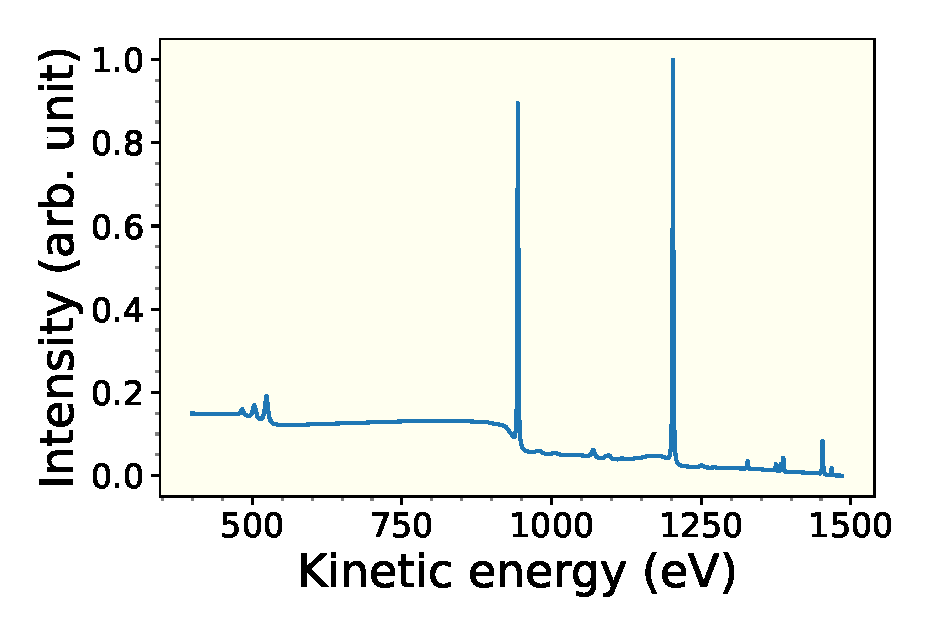
\includegraphics[width=0.99\columnwidth]{new_in.eps}
	\caption{Deep learning model.}
	\label{test1in}
\end{figure}


\begin{figure}
	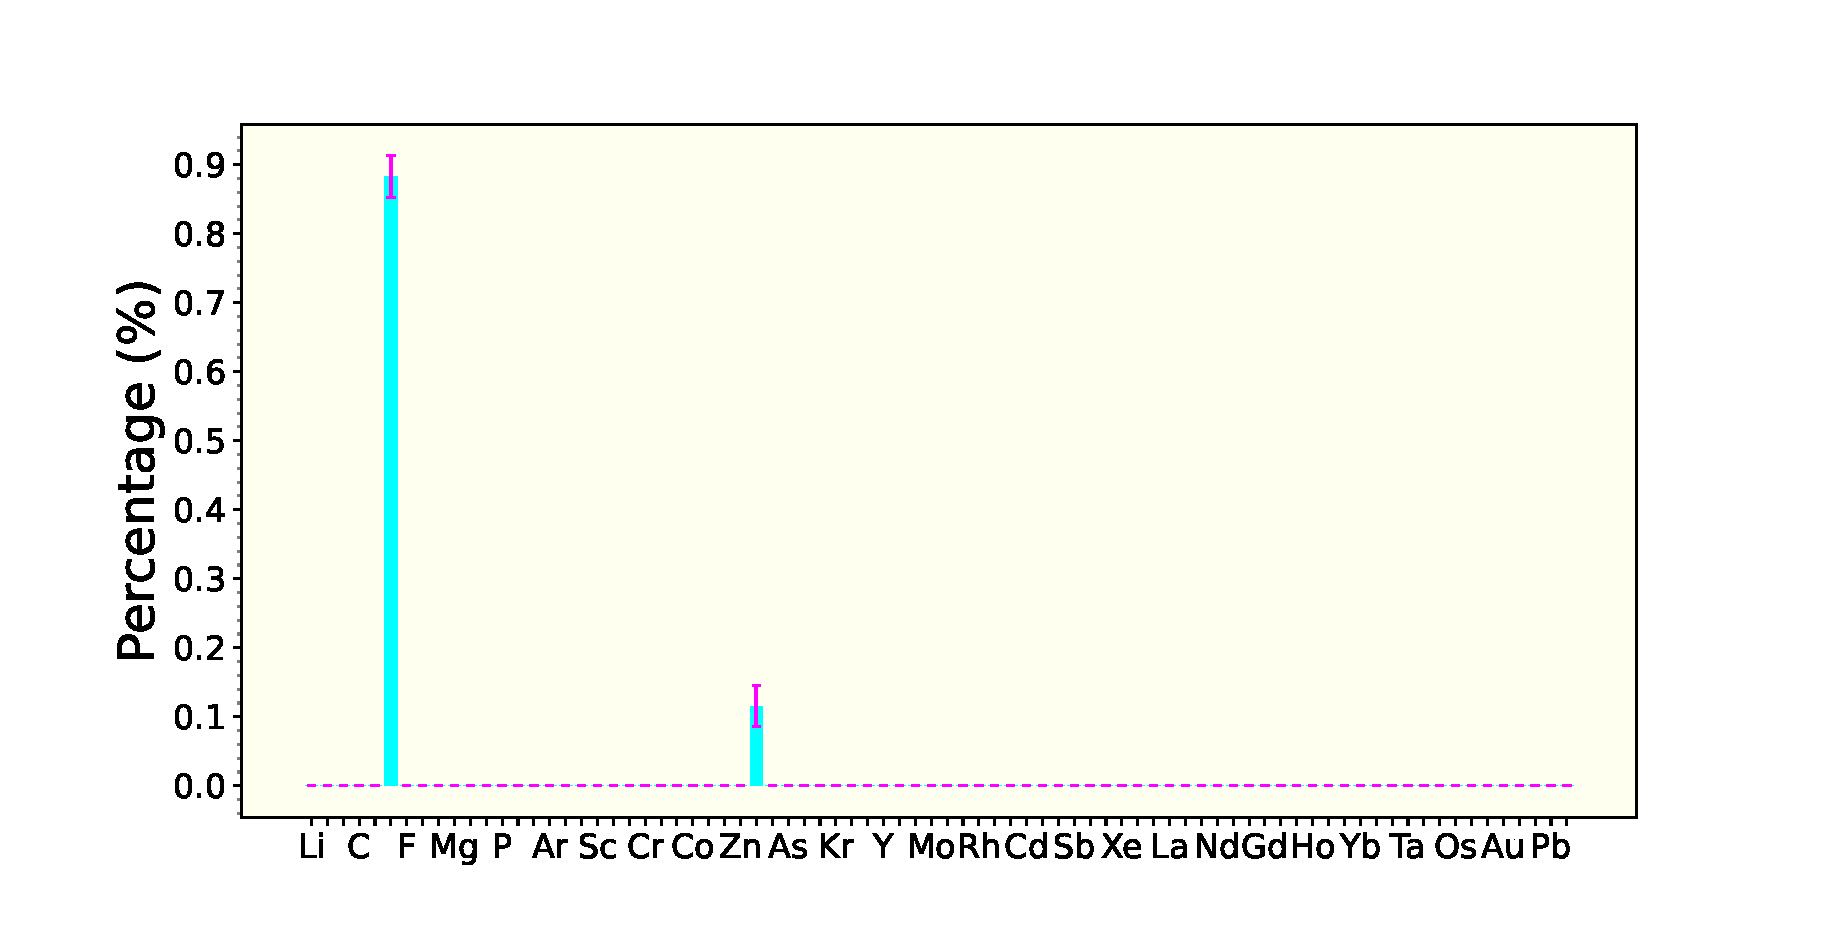
\includegraphics[width=1.15\columnwidth]{new_out.eps}
	\caption{Deep learning model.}
	\label{test1out}
\end{figure}




\end{document}
Comparison of data for a spectrum calculated and a spectrum predicted with neural network for the same, randomly selected composition.

The logarithm essentially makes the error profile more flat, reducing the impact of the larger values. 
The plus one evades the logarithm, producing negative values for errors between zero and one. 
It’s important to note that this metric assumes non-negative target variables. 
As a result, the previously seen overwhelming effect of large values is reduced, producing a more equal emphasis on data points.

MSLE measures the average squared logarithmic difference between the predicted and actual values.
MSLE treats smaller errors as less significant than larger ones due to the logarithmic transformation.


A custom loss function is show below:
\begin{equation}
	L(\{y_e\}, \{y_e^t\}) = \sum_{e=1}^{81} (y^t_{e})^2 (y_{e}-y^{t}_{e})^2, 
	\label{eq:3}
\end{equation}
where $\{y_e\}$ are the network outputs and $\{y_e^t\}$ the target values. 
%This loss function, which multiplies the standard $L_2$ norm by the net results squared, is then larger for large output values; for this reason we termed it 'high-pass filter' loss. 


In Fig.	\ref{fig1}, we show the calculated spectra maxima(at a fixed photon flux) of pure elements without contamination(labeled $\{T_e\}$), as a reference for the relative XPS intensity.
We used as labels for the regression the normalized quantification intensity defined as
\begin{equation}
	\bar{y}_e = \bar{q}_e T_e  \left ( \sum_{e=1}^{81}  \bar{q}_e T_e   \right)^{-1},
	\label{eq:1}
\end{equation}
where now $\bar{y}_e$ is the contribution of the element $e$ to the total intensity spectrum\cite{drera2020deep}. 

In order to obtain the actual quantification $(\{q_e\}, e = 1, \ldots, 81.)$ of the elements, we post-process the learned outputs of the network.
\begin{equation}
	q_e = y_e  /T_e \left ( \sum_{e=1}^{81}  y_e   \right)^{-1}. 
	\label{eq:2}
\end{equation}


\begin{figure}
	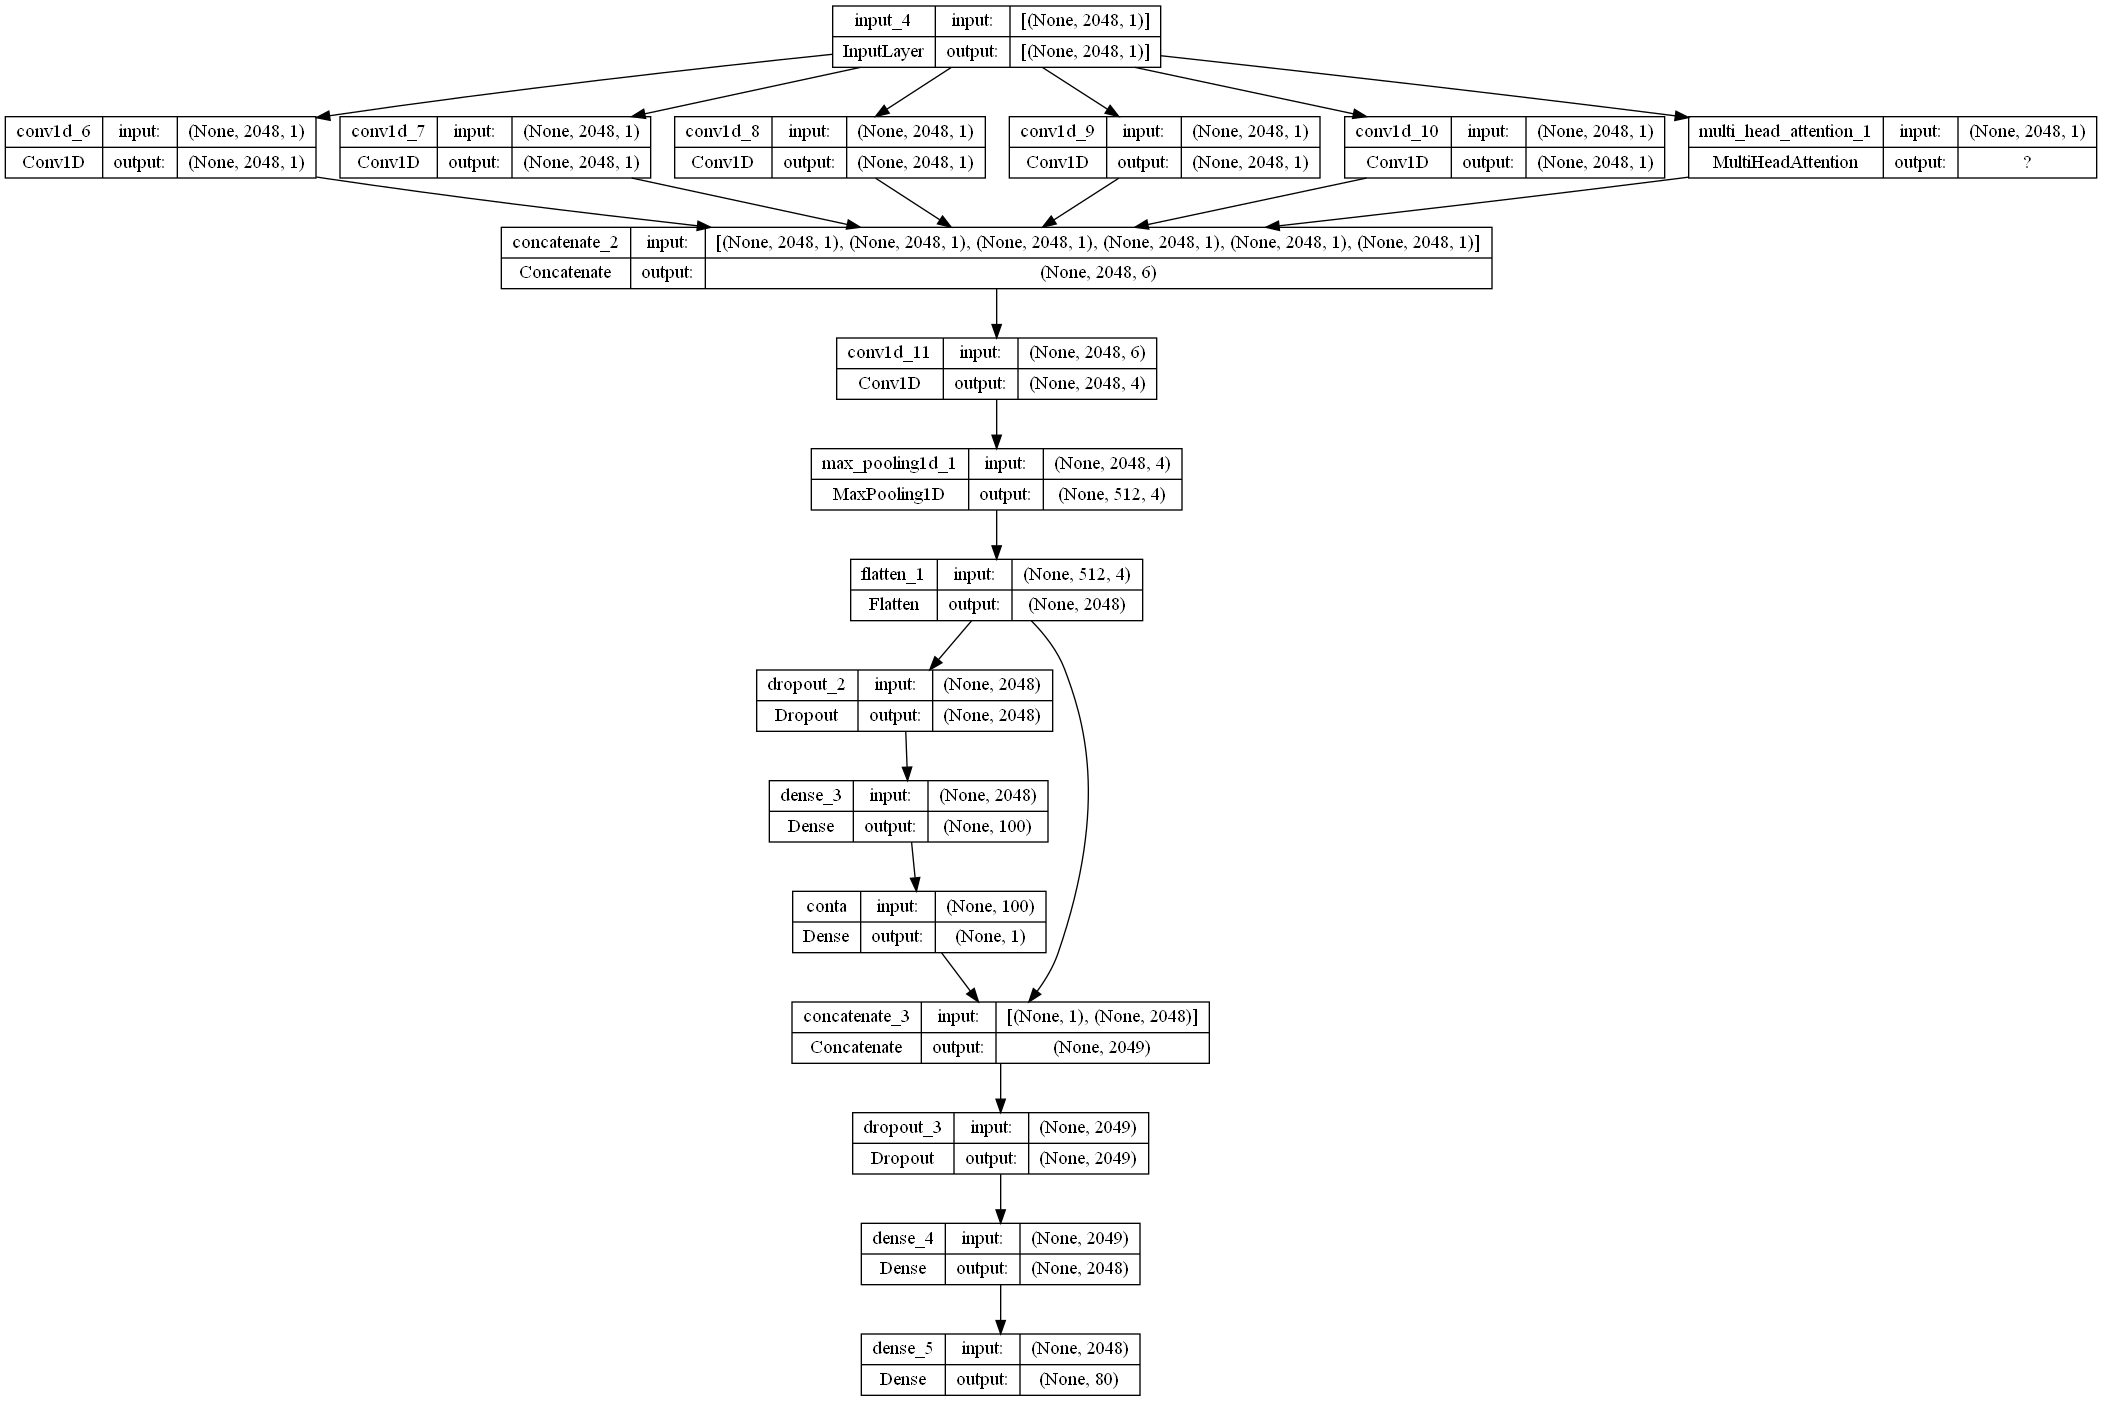
\includegraphics[width=1.\columnwidth]{model_plot.png}
	\caption{Deep learning model. Total number of trainable parameters is  4569323.}
	\label{model}
\end{figure}


\begin{figure}
	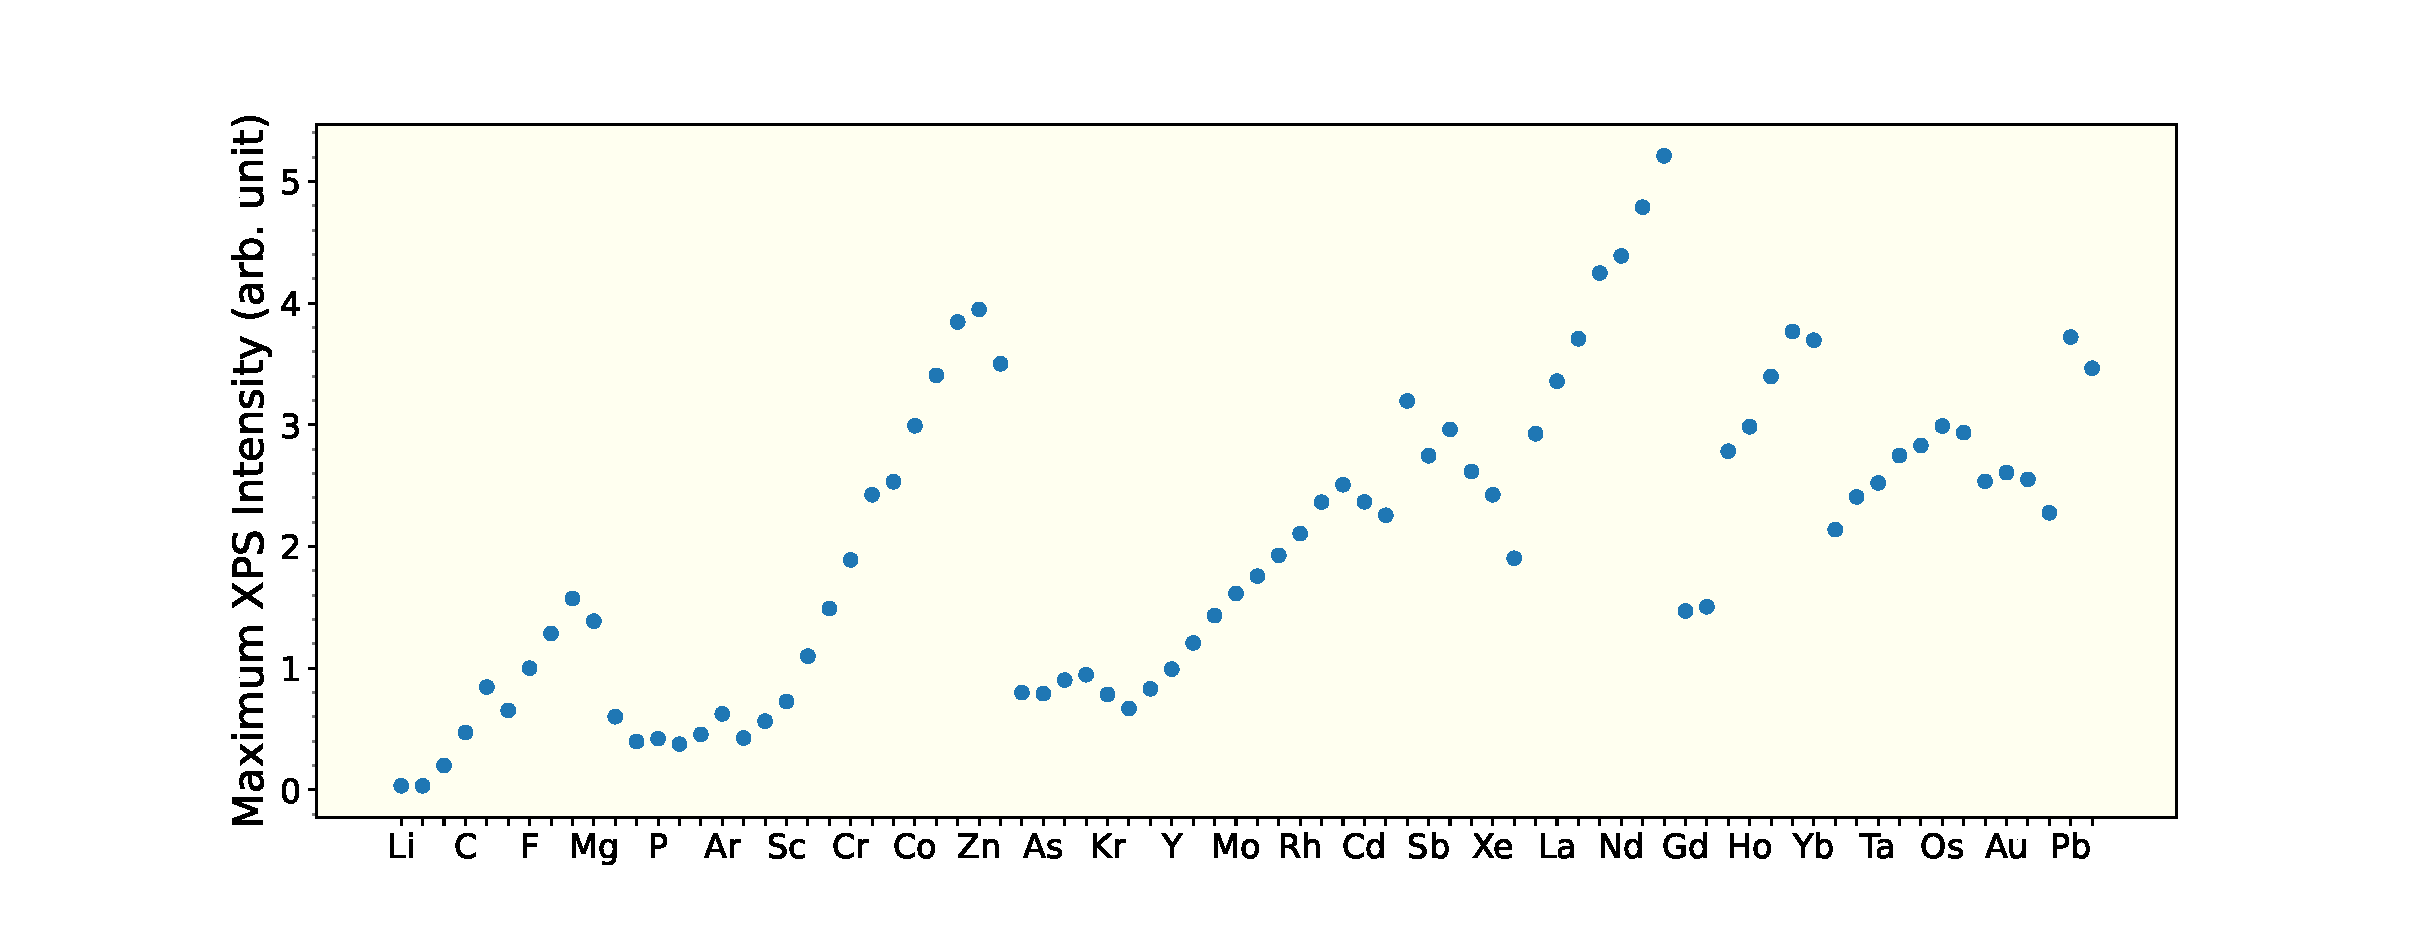
\includegraphics[width=1.15\columnwidth]{my_plot1.eps}
	\caption{Maximum XPS intensity ($\{T_e\}$) of simulated spectra for each pure element.  Along the x-axis, we have listed the atoms in order of atomic number.}
	\label{fig1}
\end{figure}

%To compare the performance of the deep learning model in the test set

 %(loss: Huber loss function, delta=0.08). 
%Huber loss is an objective function used in regression, 
%that is less sensitive to outliers in data than the squared error function.